\chapter{General Setup}\label{ch:general_setup}

This chapter describes the implementation of the offloading framework in use. However, since this thesis conducts experiments both in simulation and on real robot, there are technical differences between the actual software setups. To avoid redundancies, this chapter introduces the general offloading setup in \cref{sec:general_setup:implementation} that is mutually adopted by the two setups. Furthermore, \cref{sec:general_setup:offloading_strategies} also describes the algorithms that are used to realize different offloading strategies. 
Finally, in \cref{sec:general_setup:evaluation}, this chapter discusses the evaluation paradigm in use for different evaluation metrics.

\section{Implementation}\label{sec:general_setup:implementation}

This thesis implements an offloading pipeline for a robotic object detection task. This includes an offloading module making decision whether to offloading the image from the camera sensor to the edge computer or to compute the image locally using onboard resources. An inference pipeline for object detection task is implemented using pre-trained models from YOLOv5 \cite{Jocher2022} deployed using PyTorch library \cite{Paszke2019}. Furthermore, in order to test the offloading framework in repeatable and comparable experiments, a simulated scenario is implemented in \gls{gazebo} \cite{Koenig2004} and a recording of the scenario run is created with \gls{ros}. Finally, since the output of the object detection task is not used in any downstream applications. This thesis considers and implements various evaluation paradigms to retrieve meaningful results from the data collected during the experiments. To delimit, this thesis only investigates the scenario where one \gls{amr} offloads to one edge computer. Investigations for multi-robot multi-edge scenarios are beyond the scope of this thesis. 

\subsection{Offloading Module}

\begin{figure}[htp]
    \centering
    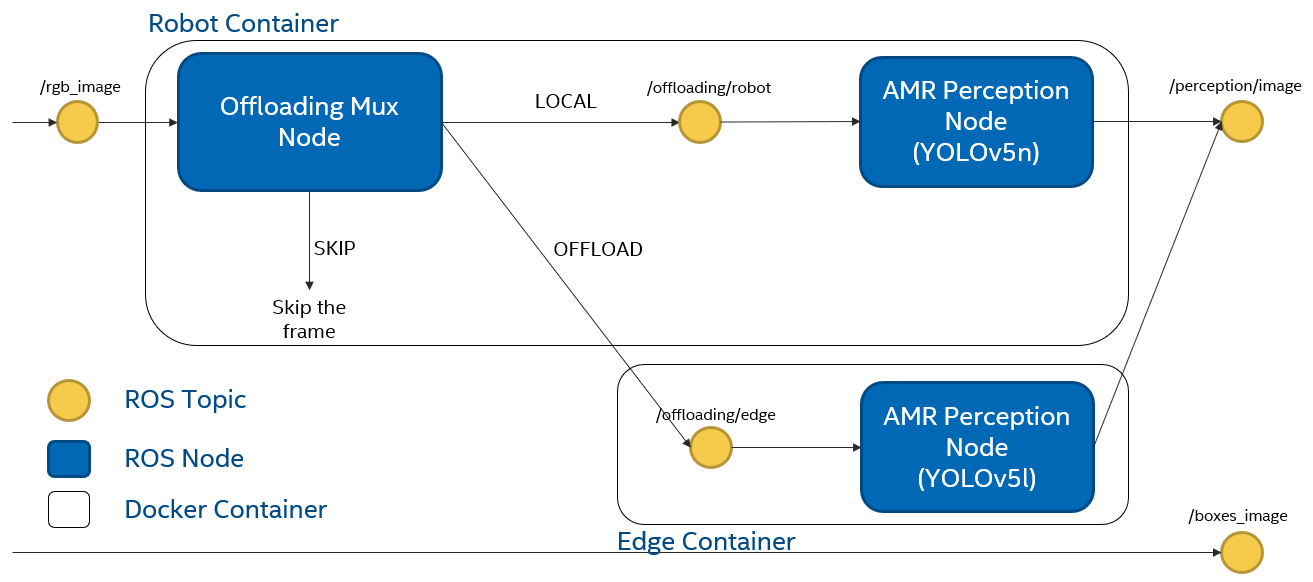
\includegraphics[width=120mm]{figures/setup/general_setup.png}
    \caption{General Setup (TODO: adapt this image)}
    \label{fig:general_setup}
\end{figure}

% TODO: this may need some adaptions to the dynamic offloading module
An offloading pipeline should have the abilities to make decision, coordinate the resources and communicate over the network. A generic offloading pipeline is illustrated in~\cref{fig:general_setup}. Each blue block represents a \gls{ros} node and each yellow circle represents a \gls{ros} topic. The arrows indicate the directions of the data flow. The dotted lines are the virtualization of the robotic system and the edge computer. The images can come from either a camera sensor or the replay of the simulated scenario. Once the \gls{amr} receives the image, the offloading module will have to decide whether to offload the image to the edge computer or pass it to the local perception node, which uses a simpler and lighter model for image inference. The offloading module makes offloading decisions by publishing the received image to pre-defined \gls{ros} topics. Once the perception nodes receive the image, they will start to do inference on the given image. Then, the processed results are published to another pre-defined \gls{ros} topic and recorded by the \gls{ros} bag. Meanwhile, the ground truth of the simulation for the object detection task is also published to a \gls{ros} topic and recorded by the \gls{ros} bag. 

In order to evaluate different offloading strategies, the offloading module possesses the ability to switch between them. Therefore, the offloading strategies act as plugins for the offloading module. Furthermore, the offloading module is responsible for loading the static hyper-parameters for the offloading strategies on start-up and also for keeping track of the run-time states of the system to allow dynamic offloading strategies. In an offloading pipeline, the system states come from various \gls{ros} nodes observing different functionalities of the system. This information is published to different \gls{ros} topics and subscribed by the offloading module. To reduce the influence of the fluctuation in the observed system states, the offloading module applies a \gls{sma} algorithm to smooth the data. 

Since the offloading pipeline is built upon the \gls{ros}, the behaviour of \gls{ros} and its underlying technical realization is crucial to the behaviour of the offloading pipeline, such as \gls{dds} and \gls{qos} settings. The exact influence of these settings on the behaviour of the offloading pipeline and the performance of the offloading will be discusses in \cref{ch:simulation} and \cref{ch:real_robot_experiment}. 

\subsection{Perception Module}

% discuss the choice of synchronous inference and asynchronous inference. Also defend not retraining the model.

% TODO: find the quote on the edge computers
In general, an offloading task can be any computationally intensive algorithms the \gls{amr} is required to run, such as perception, navigation, \gls{slam}, path planning, etc. This thesis chooses an object detection task as an example, because an object detection task can have significant performance difference between the \gls{amr}'s onboard system and the edge computer, which corresponds to the usage scenario of the edge offloading. An \gls{amr} is usually equipped with a simple onboard system with only access to \gls{cpu}, while an edge computers are usually cloudlets and data centers on premise with access to \gls{gpu}. As mentioned in \cref{ch:background}, the \glspl{amr} use primarily \glspl{dnn} to detect objects. With frameworks like PyTorch that can make use of the \gls{gpu}, the performance difference between \gls{amr}'s onboard system and the edge computer is immense. Therefore, this thesis chooses the object detection as an example for offloading tasks. 

% TODO: fill in the real value
\begin{table}[htb]%
    \centering%
    \begin{tabular}{lccccc}
        \toprule
        Model &                     YOLOv5n &   YOLOv5s &   YOLOv5m &   YOLOv5l &   YOLOv5x \\
        \midrule
        Robot inference time &      0.0 ms &    0.0 ms &    0.0 ms &    0.0 ms &    0.0 ms  \\
        Edge inference time &       0.0 ms &    0.0 ms &    0.0 ms &    0.0 ms &    0.0 ms  \\
        Model size &                0 MB &      0 MB &      0 MB &      0 MB &      0 MB    \\
        \gls{map} &                 45.7\% &  56.8\% &    64.1\% &    67.3\% &    68.9\%  \\
        \bottomrule
    \end{tabular}
    \caption{Inference times of different YOLOv5 models on \gls{amr}'s onboard system and edge computer}
    \label{tab:inference_time}%
\end{table}

% TODO: ask if it's okay to list the hardware specification
% TODO: better phrasing
In order to adapt to the performance difference between the \gls{amr}'s onboard system and the edge computer, the perception module should have two models available for object detection: a lightweight model that runs on the onboard system and a more complex model that runs on the edge computer. \gls{yolov5} provides a series of models with different complexities. To find appropriate models for the onboard system and the edge computer, this thesis investigates the inference times of different models on different machines, which can be taken from \cref{tab:inference_time}. To simulate the computation capability discrepancy between the two systems, this experiment uses a \gls{nuc} equipped with an Intel(R) Core(TM) i3-8109U \gls{cpu} and without access to \gls{gpu}. On the other hand, the edge computer is equipped with an Intel(R) Core(TM) i9-7900X \gls{cpu} and equipped with Nvidia GeForce GTX 1060 6GB \gls{gpu}. The models are deployed with \gls{pytorch} and output an array of bounding box detections. The inference time is measured between the time when the \gls{yolov5} receives the image and the time when the perception node outputs an array of bounding box detections. This includes the time for image pre-processing and the time of results post-processing. Furthermore, the image input for the offloading module has a frame rate has an average of 30 frames per second. To achieve real time, it is necessary that the inference time does not exceed 100 ms (\textbf{\textit{maybe phrase it better here}}). Longer inference time also cause the actual precision of the object detection to deteriorate, which will be discusses in \cref{sec:general_setup:evaluation}. The model sizes and the \gls{map} data are taken from the the documentation from \citeauthor*{Jocher2022} \cite{Jocher2022}. The \gls{map} data are evaluated on \gls{coco} val2017 \cite{Lin2014}. As a compromise between the inference time and the performance, this thesis chooses to deploy \gls{yolov5}n on the \gls{amr}'s onboard system and \gls{yolov5}l on the edge computer. 

To delimit, the object detection models in use are pre-trained and not re-trained with custom data from the simulation. This thesis intends to investigate different offloading strategies and generating custom data-sets and re-training the models are laborious tasks. Therefore, a re-training of the models is beyond the scope the this thesis. \citeauthor*{Jocher2022} \cite{Jocher2022} state that the all pre-trained models are trained on \gls{coco} data-sets for 300 epochs with default settings. Moreover, this thesis only considers human obstacles, which is a detection class in \gls{coco} data-sets. Therefore, the pre-trained models can provide comparability between different offloading strategies on different machines. Furthermore, re-training of the models is dependent on the quality and the size of the custom data-sets. An improper re-training can introduce additional errors or over-fitting of the models and thus undermine the comparability. 

\subsection{State Monitor}

To evaluate different offloading strategies, this thesis need to get access to the system states, such as the \gls{cpu} usage, energy consumption, and network bandwidth. Various modules are implemented to measure them. 
The measurements from these modules are recorded for evaluation and also used for dynamic strategies that making decision based on run-time states of the system. However, in simulation experiments, the virtualization of the \gls{amr}'s onboard system and the edge computer is realized by the \gls{docker} containers. In contrast, different physical computers are used in the real-robot experiments. This difference in the system virtualization affects how the system states are measured. 

For simulation experiments, \gls{docker} provides the containerized system virtualization and virtual network interfaces. \citeauthor*{Ruggeri2022} \cite{Ruggeri2022} proposes that the network bandwidth in use can be measured with the network throughput. The network throughput and \gls{cpu} usage can be measured with the the statistics of the \gls{docker} containers, which is a functionality provided by \gls{docker}. Alternatively, the system states of containers can be monitored using \gls{cadvisor}. For real-robot experiments, the \gls{cpu} usage and the network throughput are measured separately on different machines using \gls{psutil} tools. In the case of Intel \glspl{cpu}, the power consumption can be measured with \gls{rapl} provided by \gls{linux} kernel Power Capping Framework. \citeauthor*{Xie2021} \cite{Xie2021} propose that the execution latency of the offloading task consists of two components: the network delay and the inference time. The network delay measures the time needed for transferring the data from the offloading module to the perception module, while the inference time measures the time the perception module need to process the inference, including the time for image pre-processing and result post-processing. The execution latency is measured with timers residing in the offloading module and and the perception module. The timers record the time stamps to critical time points in the transfer and inference process and calculate the time difference. Then, the data are published to a \gls{ros} topic and can be access by other subscribers. 

% TODO: not sure if this paragraph is necessary
Since it is assumed that the edge computer has abundant resources, the system states of the edge computer are not measured and are not taken into consideration during the decision-making and the evaluation process. Furthermore, even though this thesis only investigates the single-robot single-edge scenario, the available resources from the edge computers can be affected by numerous factors in real-world applications, such as the number of edge computers, the number of \glspl{amr}, and other processes running the edge computers. In addition, with more powerful hardware and easy access to power supply, the edge computer consumes more energy and computation resources for the same task than the \gls{amr}'s onboard system. Therefore, it is pointless to compare the consumption of the resources between two systems with na\"{i}vet\'{e}. In contrast, the network connection between the \gls{amr} and the edge computer is fragile and prone to disturbance. Therefore, this thesis only considers the system states of the \gls{amr}'s onboard system and the network condition between the \gls{amr} and the edge computer. 

\subsection{Offloading Strategies}\label{sec:general_setup:offloading_strategies}

Offloading strategies decides how the \gls{amr} offloads the computation task to the edge computer and have influence on various metrics of the system. Therefore, they are the core of the this thesis. As baselines, this thesis first investigates the scenarios where the \gls{amr} only computes the object detection task locally on its onboard system or only offloads the task to the edge computer. Then, the thesis continues to investigate the scenarios where the \gls{amr} offloads a portion of the frames with a fixed ratio. The offloading strategies with a fixed offloading ratio can be realized with \cref{alg:ratio_strategy}. The offloading ratio should be a value ranging from 0 to 1. Any offloading ratios greater 1 will cause the offloading module only to offload to the edge computer. Accordingly, any negative offloading ratios will cause the offloading module only to compute locally. With results from the experiments on baseline offloading strategies, this thesis intends to find the limits of the system and analyze its behaviour. 


% This sections describes how RobotOnlyStrategy, EdgeOnlyStrategy, RatioStrategy are implemented. Include a psuedo algorithms here for RatioStrategy
\begin{algorithm}[htp]
\caption{Algorithm to offload with a fixed ratio}\label{alg:ratio_strategy}
\begin{algorithmic}[1]
    \Function{RatioStrategy}{$r$} \Comment{where r is the offloading ratio}
        \State $c_1 \gets \, $GetImageCounter()\Comment{Get the counter for the total images received}
        \State $c_2 \gets \, $GetOffloadCounter()\Comment{Get the counter for the images offloaded}
        \State SetImageCounter($c_1 + 1$) \Comment{Add one first to image counter to avoid zero division}
        \If{$c_2 / c_1 \ge r$}
            \State return false \Comment{Compute locally}
        \Else
            \State SetOffloadCounter($c_2 + 1$)
            \State return true \Comment{Offload to edge computer}
        \EndIf
    \EndFunction
\end{algorithmic}
\end{algorithm}

Dynamic offloading strategies use the run-time system states to decide whether to offloading. They can adapt to the dynamic changes of the system and the network. With the results from the baseline offloading strategies, this thesis continues to investigate one dynamic strategy. More specifically, a simple version of the offloading strategy proposed by \citeauthor*{Ning2019} \cite{Ning2019} with the goal of minimizing the execution latency. Moreover, this dynamic offloading strategy is subjected to constraints of other system states. In this thesis, we consider two run-time system states as constraints: \gls{amr}'s \gls{cpu} usage and the network throughput. The problem can be formulated as a constraint optimization problem as follow:

\begin{equation}
    \min_{(\alpha, \beta)} \: t_{latency} = t_{inference} + t_{network}
\end{equation}

with

\begin{equation*}
    t_{inference} = \alpha t_{inference}^{L} + \beta t_{inference}^{E}
\end{equation*}
\begin{equation*}
    t_{network} = \alpha t_{network}^{L} + \beta t_{network}^{E}
\end{equation*}

s.t.

\begin{equation*}
    \alpha + \beta = 1
\end{equation*}

\begin{align*}
    & \alpha = \begin{cases}
        1, & \text{if the task is processed locally} \\
        0, & \text{else.}
    \end{cases} \\
    & \beta = \begin{cases}
        1, & \text{if the task is processed by the edge computer} \\
        0, & \text{else.}
    \end{cases}
\end{align*}

where the $t_{latency}$ represents the overall execution latency of the object detection task and $t_{inference}$ and $t_{network}$ represent the inference time and the network delay correspondingly. 

In addition to the execution latency, the offloading decision is also subjected to the \gls{amr}'s \gls{cpu} usage and the network throughput. If the \gls{cpu} usage exceeds certain value, the \gls{amr} only offloads to the edge. Similarily, the \gls{amr} only computes the task locally if the network throughput exceeds the threshold. These constraints ensure that the \gls{amr} and the network are capable of finish the task at all. The decision-making strategy can be implemented as 

\begin{algorithm}[htp]
\caption{Algorithm to offload with dynamic parameters}\label{alg:decision_making_strategy}
\begin{algorithmic}[1]
    \Function{DecisionMakingStrategy}{$r, params$}\Comment{offloading ratio: $r$, run-time parameters: $params$}
        \Comment{add an algorithm here.}
    \EndFunction
\end{algorithmic}
\end{algorithm}



\section{Simulation}\label{sec:general_setup:simulation}

To run experiments both in simulation and on real robots, this thesis implements a simulated scenario of a factory warehouse with one \gls{amr} and obstacles. The simulation is recorded and replayed for each experiment run to reduce the computation overhead of the simulation and to make the experiment repeatable. Furthermore, in order to compare the results from simulation and real robot, the simulation recording is used as input for both experiments under the same replay settings. 

\subsection{Simulated scenario}

% include a bird-view shot for the simulation with warehouse, robot, and human obstacles in the view.
The scenario simulates a modern-day factory warehouse, illustrated in (refer to the figure here). The simulated scenario is implemented in \gls{gazebo} with the help of a software package called "scenario execution", which the author implemented during his work at Intel Labs. The scenario consists of a factory warehouse environment and static obstacles, such as humans, boxes, shelves, and pallets, which are common obstacles in a factory warehouse. Since the object detection models are pretrained with \gls{coco} data-sets, which do not contain many of the static obstacles. The evaluation for the \gls{map} is of the object detection task is restricted only to detect the human obstacles. To clarify, the object detection models still detect all of the classes that are defined in the \gls{coco} data-sets. However, only the human class is taken into considering when calculating the \gls{map} metric during the evaluation. Since the performance difference among different \gls{yolov5} models are negligible when the scene is too simple, this thesis includes ten human obstacles in the simulated scenario to increase the complexity of the object detection task. Moreover, some human obstacles are occluded by other obstacles in the scenario. Detecting occluded objects has been proven to be a challenging task in object detection. 

\begin{figure}
    \centering
    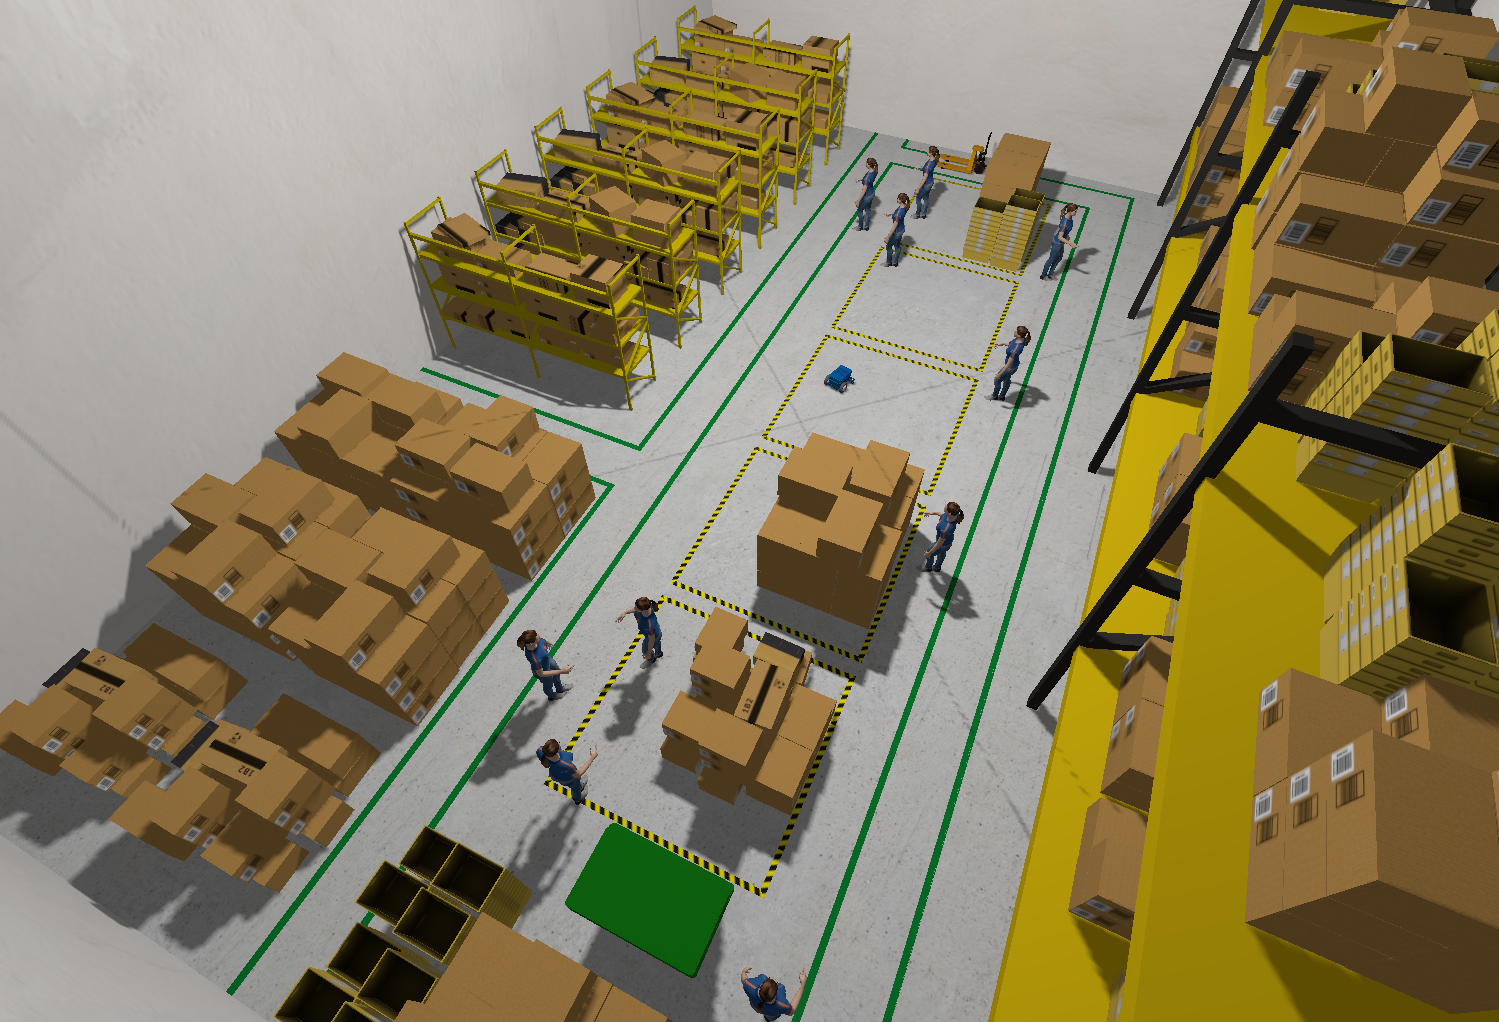
\includegraphics[width=120mm]{figures/sim/bird_view.png}
    \caption{Bird view of the simulated scenario}
    \label{fig:bird_view_scenario}
\end{figure}

The \gls{amr} is implemented as a dynamic obstacle in the scenario and it moves along a pre-defined path. The pre-define path is made up of a series of way points in the simulation. Once the \gls{amr} reaches the current way point, the scenario execution will assign the next way point to the \gls{amr}. After all way points are successfully reached, the scenario execution shuts down the simulation. In the simulation, the \gls{amr} does not collide with other obstacles. The \gls{amr} is equipped with a RGB-camera that is located on top the of the robot and facing forward. The intrinsic parameters of the RGB camera sensor is listed in \cref{tab:camera_params}. During the simulation, the camera can observe all of the obstacles in the simulation with partial occlusion of some obstacles. In addition to the RGB image stream, the simulated camera sensor also outputs a image stream that contains the ground truth for the bounding boxes in object detection task using the bounding box sensor from \gls{gazebo}. The ground truth data and the image stream are bridged from the \gls{gazebo} simulation topics to \gls{ros} topics so that the offloading pipeline can make use of them. In (cite figure of robot view here), it shows from the point of view of the \gls{amr}'s camera sensors. On the left, it shows the illustration of the bounding box ground truth data, while the image stream is shown on the right. The bounding box camera sensor and the RGB camera sensor are positioned the same and intend to simulate an actual point of view of a normal \gls{amr}.

\begin{table}[htp]
    \centering
    \begin{tabular}{lc}
    \toprule
    Parameter&                  Value\\
    \midrule
    Height&                     848 pixels\\
    Width&                      480 pixels\\
    FOV&                        1.047\\
    Frame rate&                 30 frames/sec\\
    Noise type&                 Gaussian\\
    Noise mean&                 0\\
    Noise standard deviation&   0.007\\
    \bottomrule
    \end{tabular}
    \caption{RGB camera intrinsic parameters}
    \label{tab:camera_params}
\end{table}

% describes how the robot is navigated, describes how the camera is mounted on the robot

\begin{figure}
    \centering
    \begin{subfigure}[h]{0.4\linewidth}
        \centering
        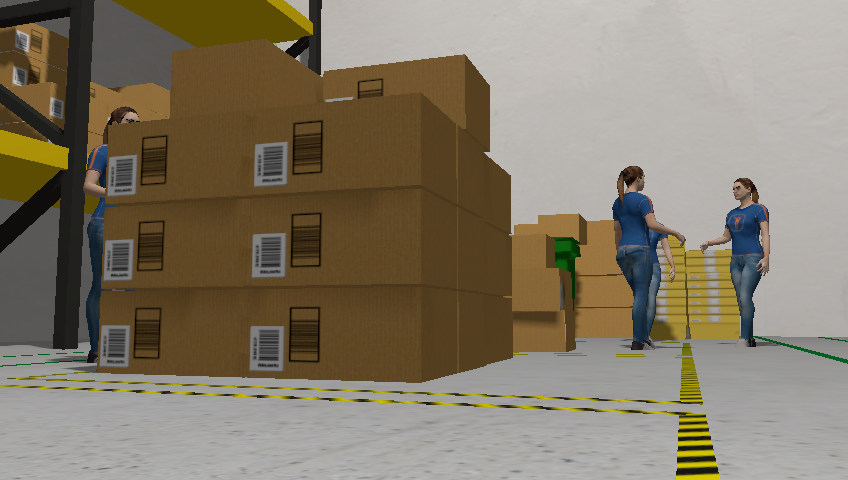
\includegraphics[width=\linewidth]{figures/sim/rgb_img.png}
        \caption{RGB image}
        \label{fig:robot_view_scenario:rgb_image}
    \end{subfigure}
    \begin{subfigure}[h]{0.4\textwidth}
        \centering
        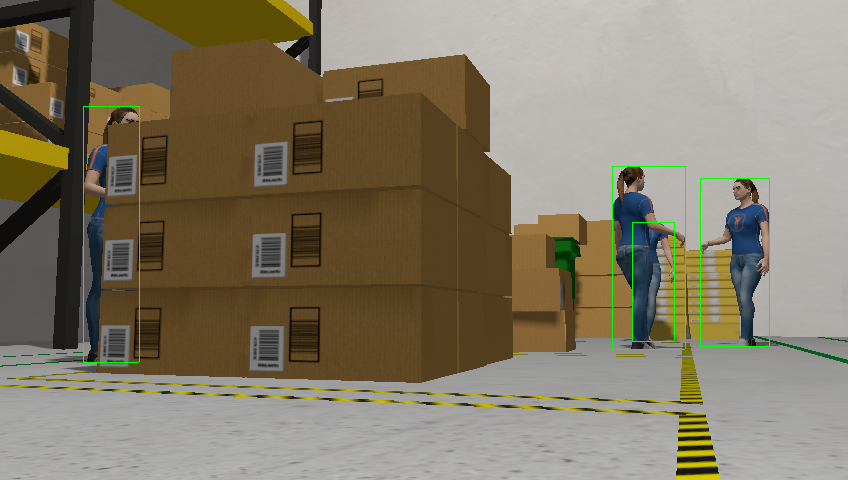
\includegraphics[width=\linewidth]{figures/sim/bbgt.png}
        \caption{Bounding box ground truth}
        \label{fig:robot_view_scenario:bbgt}
    \end{subfigure}
    \caption{Robot view of the simulated scenario}
    \label{fig:robot_view_scenario}
\end{figure}

It is worth pointing out that no dynamic obstacles are implemented in the simulated scenario. However, the \gls{amr} is dynamic and the camera sensors are mounted on top of it. Therefore, in the viewpoint of the \gls{amr}, the obstacles are constantly moving and thus could be treated as dynamic solely for the object detection task. Another reason for this is that the fresh out-of-box bounding box sensor from \gls{gazebo} is inaccurate for dynamic obstacles like humans, because dynamic human actors are implemented as the actors in \gls{gazebo} and the animation of the actors is realized by the deformation of the meshes of the actor model. Unfortunately, the bounding box sensor can only provide the bounding boxes of the undeformed actor. Therefore, the bounding boxes available are not accurate to serve as the ground truth for the object detection task. Till the finish of the thesis, the problem is not resolved with the current version of \gls{gazebo} this thesis uses. However, static human obstacles and dynamic \gls{amr} still constitutes an adequate simulated scenario for the research questions this thesis is trying to address. 

\subsection{Record and Replay}

% describes how the ROS bag is recorded and how is it replayed during the experiments and explain why this is needed. 
Simulation takes up a great amount of the resources of computers. To reduce the overhead of running the simulation alongside the experiments, this thesis records the simulation to a \gls{ros} bag and replays it during the experiment runs. This reduces the \gls{cpu} and memory usage of the host machine during the experiment and improves the performance of the rest of the offloading pipeline. As mentioned in \cref{ch:background}, \gls{ros} provides the functionality to record the topics and allows the users to replay it later, while preserving the same publishing rate and order of the messages. More importantly, this thesis conduct experiment on real robotic system with limited resources. Such system is not capable of running real-time simulation while maintaining the rest of the offloading pipeline. In real-world applications, \glspl{amr} only need to maintain the driver of the camera and minimal software to be able to get the same image input. In \cref{tab:ros_bag_comparison}, this thesis presents an experiment comparing the \gls{cpu} usage of replaying a \gls{ros} bag and running the library for the Intel RealSense camera. The results show that the two processes have the comparable \gls{cpu} usage on a robotic system. Furthermore, \gls{gazebo} slows down the simulation time compared to real time when the system is strained. Therefore, to ensure a real-time simulation, specifying a replay rate of the \gls{ros} bag can guarantee the simulation time factor is within a reasonable range. 

\begin{table}[htp]
    \centering
    \begin{tabular}{lc}
    \toprule
    Process&                    CPU usage\\
    \midrule
    \gls{ros} bag replay&       0\%\\
    RealSense camera library&   0\%\\
    \bottomrule
    \end{tabular}
    \caption{Comparison of CPU usage on robotic system}
    \label{tab:ros_bag_comparison}
\end{table}

All topics during the simulation are recorded in the \gls{ros} bag, including the RGB images, the bounding box ground truth, the camera information, etc. The image stream consists of 1748 frames and the \gls{ros} bag is replayed at around 30 frames per second during the experiment. Topics for RGB image stream and the bounding box ground truth are replayed with best effort reliability setting to ensure the RGB images are replayed the same way it is recorded. Since the \gls{ros} topics are recorded at a different time than the experiment, the time stamps of the RGB image messages and the ground truth messages have to be overwritten by the receiving time of the offloading module.

\section{Evaluation Method}\label{sec:general_setup:evaluation}

To comprehend the influence of different offloading strategies, an evaluation method on the experiment results needs to be developed. First, this thesis presents the evaluation metrics that are chosen to describe the behavior of the system. Then, this thesis discusses two evaluation methods, namely the synchronous and the asynchronous evaluation, and demonstrates why the latter is eventually chosen to evaluate the experiment results.

\subsection{Metrics}

% This section lists all the evaluation metrics used and how they are recorded and what tools are used in order to record them. 

The evaluation metrics used by this thesis fall into two categories. The second category focuses mainly on the resources of the \gls{amr}. This includes the CPU percentage, the power consumption, and the network throughput. These metrics represent the onboard resources for computation, energy, and network used by the \gls{amr}. For these metrics, this thesis also includes the results when the offloading pipeline is idling as a baseline to eliminate the influence of processes other than the perception modules on the metrics. More specifically, in the baseline, the offloading module and the perception modules are still launched and the ROS bag is also being replayed. However, the offloading module is not sending any messages to the onboard perception module or the edge perception module, i.e., there are no object detection tasks being performed at all. 

The second category describes the performance of the object detection task, including the execution latency, the overall processed frame rate, and the \gls{map}. The two components of the execution latency, i.e., the network delay and the inference time, are evaluated separately for offloading and local computation. In addition, to evaluate how the offloading pipeline is performing over the entire simulation, the overall processed frame rate, i.e., what percentage of all the frames are processed by perception modules. The \gls{map} only consider the person class in the obstacles. The detection from the perception modules is compared with the bounding box ground truth from the simulation. The evaluation algorithm is provided by the package "torchauto" as a part of the code base from \gls{amsrl}. 

For the comparison between the detection and the ground truth, the time stamps of the messages are crucial to the final result. This raises the question: what should be considered as simultaneity for the detection and the ground truth in task offloading? This thesis presents two evaluation methods of the \gls{map} metric in order to gain some insights into this question. 

\subsection{Discussion on Evaluation Methods}

In the synchronous evaluation, the detection is evaluated by being compared with the ground truth of the same time stamp. As illustrated in \cref{fig:sync_eval}, the image is either processed by the robot perception module or the edge perception module. The processed result and the ground truth are recorded by the ROS bag. After the experiment runs, the recorded result and the ground truth with the nearest time stamps are grouped as one data frame by the message filter. The message filter groups the messages from different ROS topics. The proximate messages within a time threshold can be considered as the same data frame. The threshold is currently set to 0.05 seconds. The \gls{map} is calculated within the same data frame. For the entire experiment run, the mean and the standard deviation are calculated for all the data frames. This means the data frame is discarded if no detection or ground truth is present for the specific time stamp, i.e., the \gls{map} will not be affected if the robot onboard system or the edge computer is not capable of processing the image. The capability of processing the image is however reflected in the metric of the overall processed frame percentage. 

\begin{figure}[htp]
    \centering
    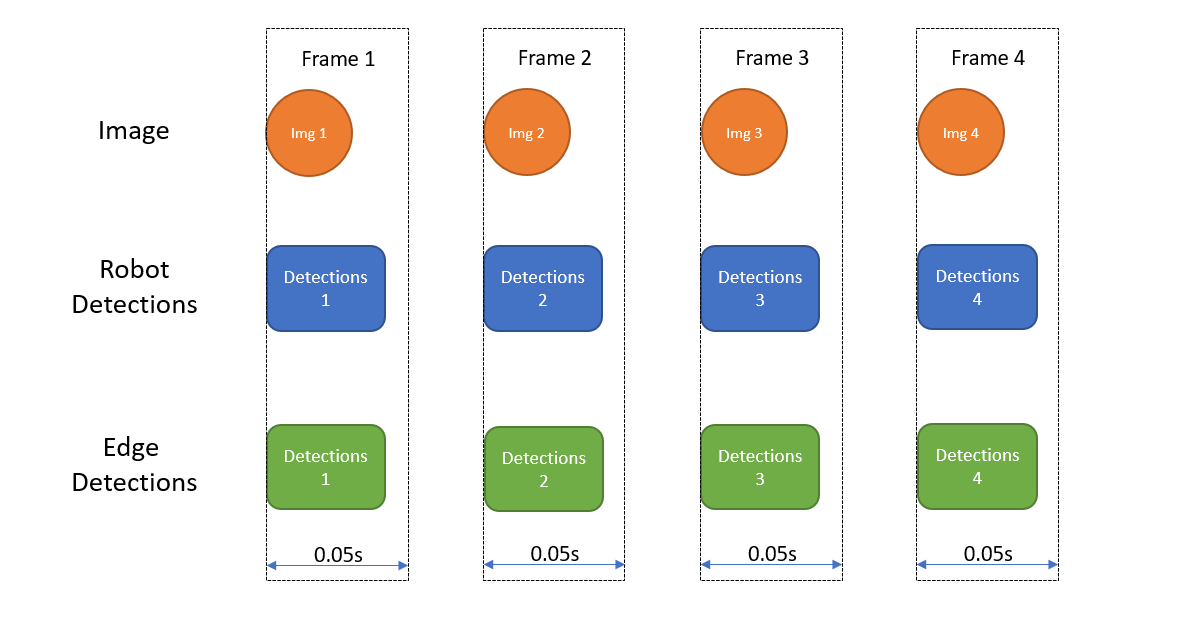
\includegraphics[width=120mm]{figures/setup/sync_eval.png}
    \caption{Synchronous evaluation}
    \label{fig:sync_eval}
\end{figure}

The synchronous evaluation method does not take the execution latency into consideration, because the detection is compared against the ground truth with the same time stamp as the original image. Therefore, the final result interpolates the \glspl{map} of the edge computer and the robot onboard system. However, this also does not represent the offloading scenario accurately. In real-world applications, the \glspl{amr} move continuously. The current situation of the \gls{amr} could be very different than the moment the image is taken by the camera if the processing takes too long and the detection is outdated. Therefore, the execution latency plays an important role in the accuracy of how well the \glspl{amr} perceives the environment. 

With the aforementioned considerations, this thesis investigates an asynchronous evaluation method that takes the execution latency into consideration, which is the evaluation method for \gls{map} metric that the thesis adopts. As illustrated in \cref{fig:async_eval}, the detection is compared against the images with the time stamps when the \glspl{amr} actually receive the processed result. This is achieved by changing the time stamps of the detection messages to the receiving time of the \glspl{amr}. Depending on how much the images have changed, the quality of the detection deteriorates with the execution latency, which is usually the case in real-world applications.

\begin{figure}[htp]
    \centering
    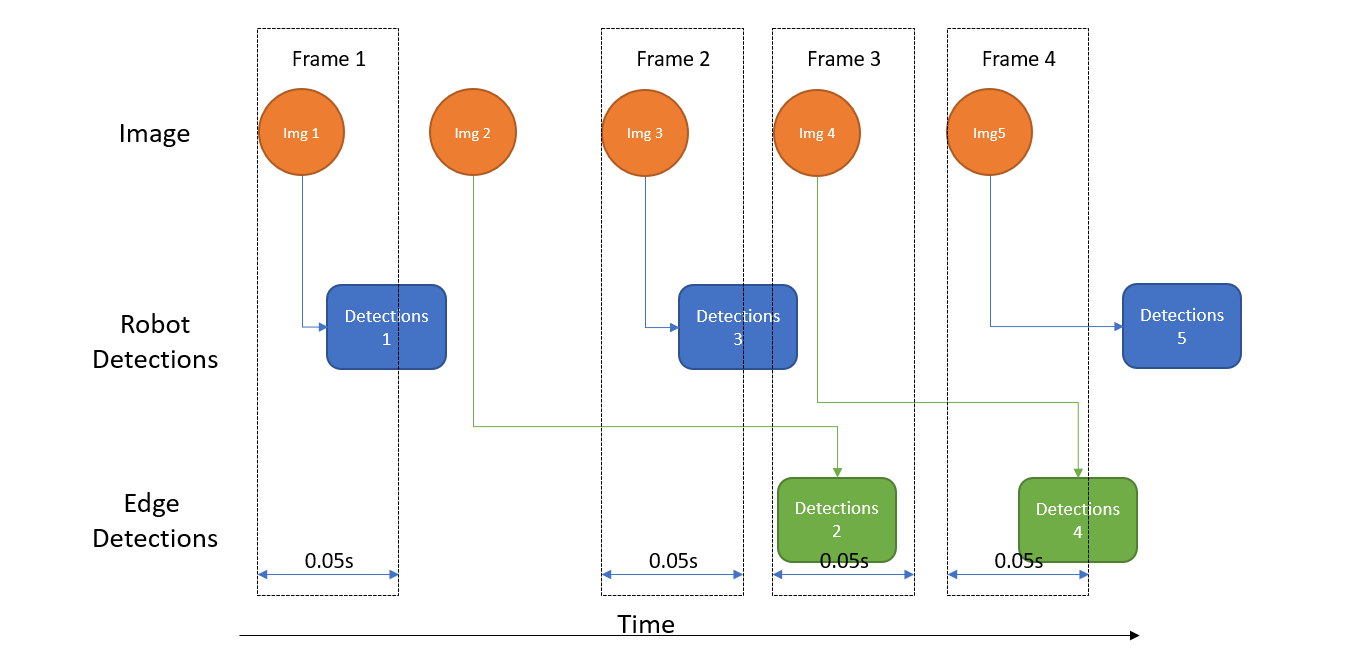
\includegraphics[width=120mm]{figures/setup/async_eval.png}
    \caption{Asynchronous evaluation}
    \label{fig:async_eval}
\end{figure}
